\documentclass[12pt,a4paper]{article}
\usepackage[utf8]{inputenc} % sempre salve seus arquivos como UTF8
\usepackage[T1]{fontenc}
\usepackage[english]{babel}

\usepackage[left=2.5cm,right=2cm,top=2cm,bottom=2.5cm]{geometry}
\usepackage{amsmath}
\usepackage{amsthm}
\usepackage{amsfonts}

\usepackage{graphicx}
\usepackage{algorithm}
\usepackage{color}
\usepackage[noend]{algpseudocode}
\usepackage{mathtools}
\usepackage{subfig}
\usepackage{diagbox}

% load times font
\usepackage{mathptmx}
\usepackage[scaled=.90]{helvet}
\usepackage{courier}

% comandos
\newcommand{\mdc}[1]{\mathrm{mdc}(#1)}

\DeclarePairedDelimiter\ceil{\lceil}{\rceil}
\DeclarePairedDelimiter\floor{\lfloor}{\rfloor}

% Foot without marker
\newcommand\blfootnote[1]{%
	\begingroup
	\renewcommand\thefootnote{}\footnote{#1}%
	\addtocounter{footnote}{-1}%
	\endgroup
}

\title{MO446 -- Introduction to Computer Vision  \\ Project 4}
\author{Breno Leite  \\ Guilherme Leite}
\date{26/10/2017}

\begin{document}

\maketitle
\blfootnote{\textit{\textbf{Important note:} The borders seen in the figures are not part of the image, they are figurative information about the starting and ending points of the image. Moreover, all the image scales in this report were changed in order to make the text more readable.}} \\

%% ---------------- Starts here --------------------------------

\textbf{\LARGE Question 3 - Image Descriptor}\\

To create a retrieval system we need to have image descriptors, in this question we extracted these descriptors for all the images in the dataset. This descriptors were saved in the disc, so the next time the program was executed it could load them, and perform faster, instead of recalculating every descriptor which is a high cost operation. \\

An image descriptor consist of all the regions in an image and their information. To extract  these regions, we firstly used OpenCV's implementation of Kmeans algorithm, to create a $k$-colored image. Figure \ref{fig:kmeans} shows the result of this image. \\

\begin{figure}[!h]
	\centering
	\subfloat[K = 2.]{
		{
			\setlength{\fboxsep}{1pt}
			\setlength{\fboxrule}{1pt}
			\fbox{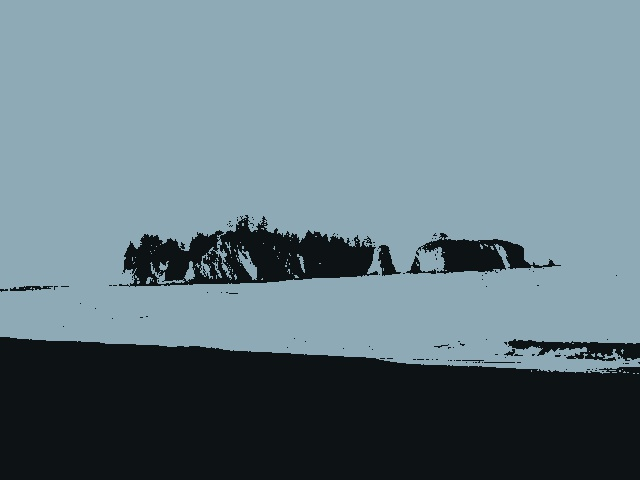
\includegraphics[scale=0.3]{report/p4-3-0-K02}}
		}
		\label{fig:kmeans02}
	}
	\quad
	\subfloat[K = 5.]{
		{
			\setlength{\fboxsep}{1pt}
			\setlength{\fboxrule}{1pt}
			\fbox{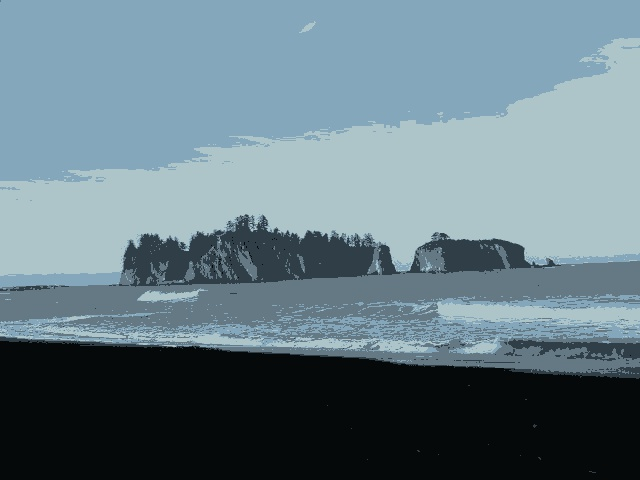
\includegraphics[scale=0.3]{report/p4-3-0-K05}}
		}
		\label{fig:kmeans05}
	}
	\quad
	\subfloat[K = 8.]{
		{
			\setlength{\fboxsep}{1pt}
			\setlength{\fboxrule}{1pt}
			\fbox{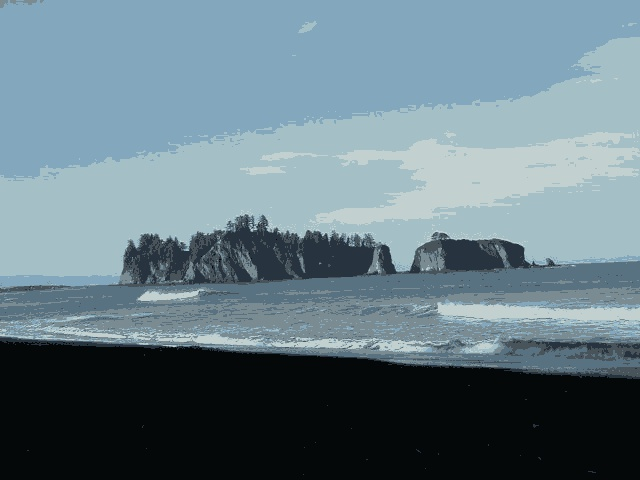
\includegraphics[scale=0.3]{report/p4-3-0-K08}}
		}
		\label{fig:kmeans08}
	}
	\quad
	\subfloat[K = 10.]{
		{
			\setlength{\fboxsep}{1pt}
			\setlength{\fboxrule}{1pt}
			\fbox{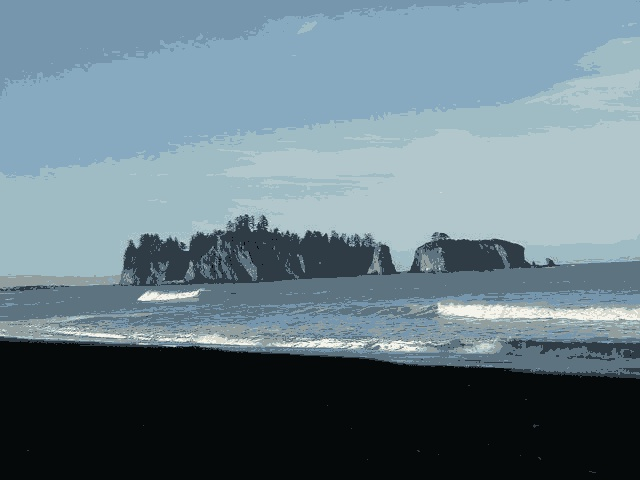
\includegraphics[scale=0.3]{report/p4-3-0-K10}}
		}
		\label{fig:kmeans10}
	}
	\caption{$K$-colored image formed by the kmeans algorithm}
	\label{fig:kmeans}
\end{figure}

The algorithm returns $K$ regions extracted based on their pixel intensity, in Figure \ref{fig:kmeans} each color represents a region. The number of regions ($K$) was selected by trial and error, a small $K$ yields big generic regions, as in Figure \ref{fig:kmeans02} for example the sky and the ocean were blended into a single region, which is not helpful to discriminate between images. In contrast a big $K$ yields to many small regions as seen in Figure \ref{fig:kmeans10}, small regions don't increase matching accuracy, the reasoning about it will be explained later on, although they increase the computation time significantly. A $K = 5$ yielded to better results, as seen in Figure \ref{fig:kmeans05}, and the rest of the work will be using this value. \\

A comparison between the sky in Figure \ref{fig:kmeans05} and Figure \ref{fig:kmeans08} shows a reasoning for the better results using $K = 5$, in Figure \ref{fig:kmeans05} it is possible to distinguish around two colors for the sky region, a light and a dark blue, as in Figure \ref{fig:kmeans08} the sky was sub-divided into roughly three regions, but a pixel by pixel analysis reveals more regions describing the sky which won't really improve the matching process and would make the algorithm less time efficient. \\

The ideal $K$ value can vary from image to image, and there is a method to choose the best value depending on a set of tests, this method is called silhouette analysis and we did not explored this automatic approach in this project. \\

In order to use these regions as an image descriptor, it is desired that descriptive enough regions. The regions returned by Kmeans are still too generic, some of them are even disconnected, as in Figure \ref{fig:kmeans05} the sky and some waves are in the same region, even though they are disconnected and represent different objects in the scene. \\

To eliminate these disconnected regions we ran a Breadth-first search (BFS) in the entire image. The BFS obtains the connected regions separately, which receives a new label, eliminating disconnected regions altogether, Figure \ref{fig:bfs} shows the new regions generated by the algorithm. The borders remained unchanged during this process, but reducing their noise could improve the expression of some regions, increasing the accuracy of the solution. \\

\begin{figure}[!h]
	\centering
	\subfloat[X = 0.]{
		{
			\setlength{\fboxsep}{1pt}
			\setlength{\fboxrule}{1pt}
			\fbox{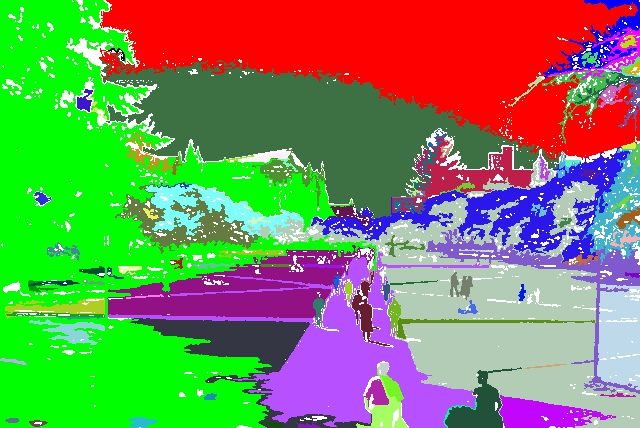
\includegraphics[scale=0.3]{report/p4-3-1-X00}}
		}
		\label{fig:bfs00}
	}
	\quad
	\subfloat[X = 6.]{
		{
			\setlength{\fboxsep}{1pt}
			\setlength{\fboxrule}{1pt}
			\fbox{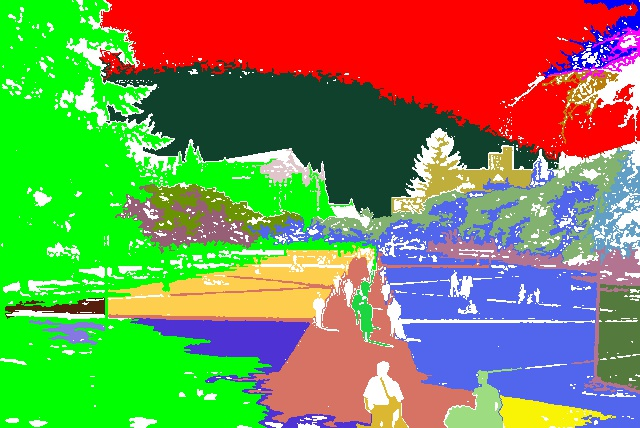
\includegraphics[scale=0.3]{report/p4-3-1-X06}}
		}
		\label{fig:bfs06}
	}
	\quad
	\subfloat[X = 10.]{
		{
			\setlength{\fboxsep}{1pt}
			\setlength{\fboxrule}{1pt}
			\fbox{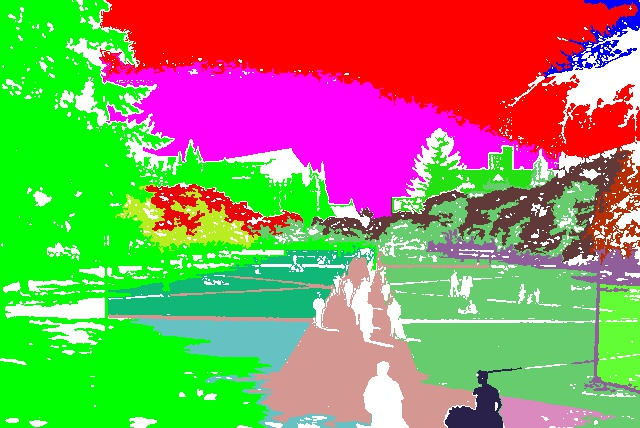
\includegraphics[scale=0.3]{report/p4-3-1-X10}}
		}
		\label{fig:bfs10}
	}
	\quad
	\subfloat[X = 20.]{
		{
			\setlength{\fboxsep}{1pt}
			\setlength{\fboxrule}{1pt}
			\fbox{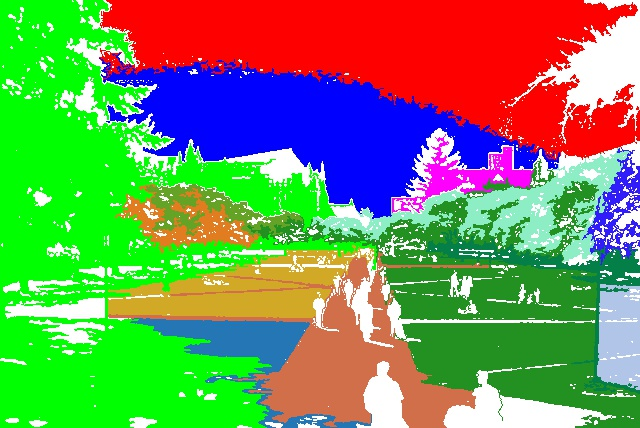
\includegraphics[scale=0.3]{report/p4-3-1-X20}}
		}
		\label{fig:bfs20}
	}
	\caption{Connected regions extracted using the BFS explorer for different $X$ values.}
	\label{fig:bfs}
\end{figure}

In Figure \ref{fig:bfs} each color represents a connected region and Figure \ref{fig:bbox} shows their bounding boxes. Regions that are too small don't really describe enough of a feature to be relevant, and thus are discarded, in Figure \ref{fig:bfs} the white color is used to represent the discarded regions. \\

\begin{figure}[!h]
	\centering
	\subfloat[X = 0.]{
		{
			\setlength{\fboxsep}{1pt}
			\setlength{\fboxrule}{1pt}
			\fbox{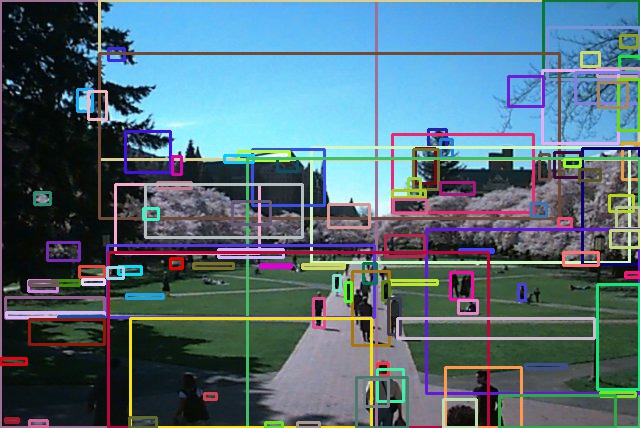
\includegraphics[scale=0.3]{report/p4-3-2-B00}}
		}
		\label{fig:bbox00}
	}
	\quad
	\subfloat[X = 6.]{
		{
			\setlength{\fboxsep}{1pt}
			\setlength{\fboxrule}{1pt}
			\fbox{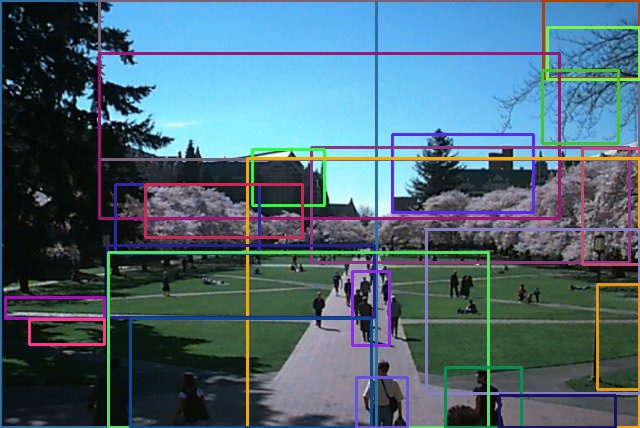
\includegraphics[scale=0.3]{report/p4-3-2-B06}}
		}
		\label{fig:bbox06}
	}
	\quad
	\subfloat[X = 10.]{
		{
			\setlength{\fboxsep}{1pt}
			\setlength{\fboxrule}{1pt}
			\fbox{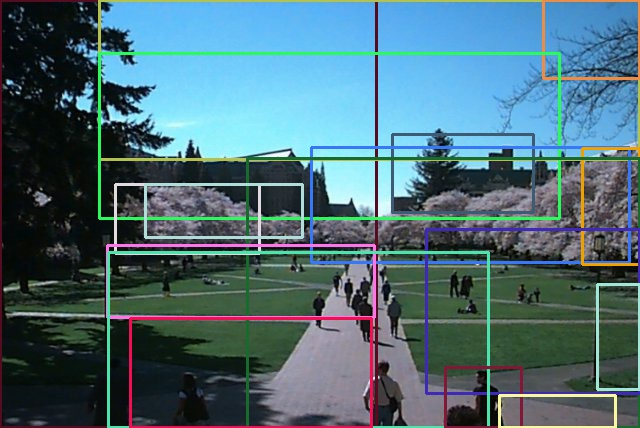
\includegraphics[scale=0.3]{report/p4-3-2-B10}}
		}
		\label{fig:bbox10}
	}
	\quad
	\subfloat[X = 20.]{
		{
			\setlength{\fboxsep}{1pt}
			\setlength{\fboxrule}{1pt}
			\fbox{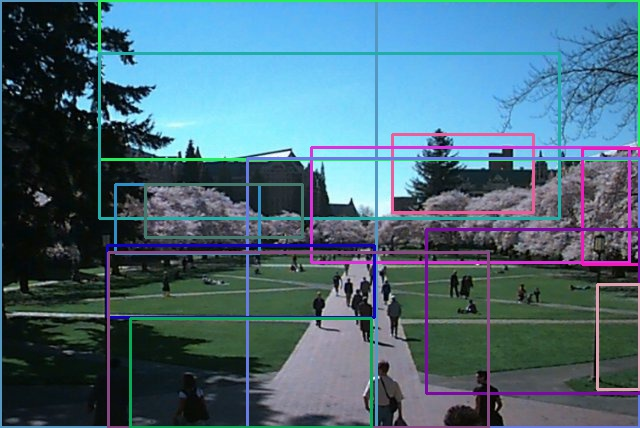
\includegraphics[scale=0.3]{report/p4-3-2-B20}}
		}
		\label{fig:bbox20}
	}
	\caption{Bounding box of each region calculated with different $X$ values.}
	\label{fig:bbox}
\end{figure}

A region is considered too small if its size is smaller than the multiplication of a factor $X$ by the average region size, this value was chosen based on our analysis of the yielded results given by the input dataset. \\

In Figure \ref{fig:bfs00} and Figure \ref{fig:bbox00} the value of $X$ is set to zero and it is possible to observe regions as big as one pixel line being taken, which is counter productive towards our goal as they don't describe something relevant. In Figure \ref{fig:bfs06} and Figure \ref{fig:bbox06}, with $X = 6$, smalls non-discriminative regions are still being selected, like the tree on the right upper side of the image, the human carrying a bag in the bottom center (Figure \ref{fig:bfs06} shows that only the bag and pants were selected) and a few smalls patches of grass in the left bottom side, all of those describes non-discriminative features that could hurt the final result. \\

In Figure \ref{fig:bfs10} and Figure \ref{fig:bbox10}, where $X = 10$, there are still some non-discriminative regions being selected, like half of the tree in the right upper corner, but they are few and contrasted with a majority of somewhat big, discriminative regions, like the cherry trees, the buildings in the back and the path in the center. In Figure \ref{fig:bfs20} and Figure \ref{fig:bbox20}, with $X = 20$, almost all the small ignorable regions were discarded and it performed well in this image, but since it was a big value it could start eliminating discriminative regions on other images, this and the inefficiency of the small values to determine good sized regions was the reason why we chose $X = 10$. \\


These regions will be used as descriptors of the image, and compared later on, to do so it is necessary to describe each region, in a data structure,  a feature vector with the following information were used: region size, region mean color, region centroid, and some texture features for the region patch. The patch of the texture features were extracted using the delimitations of their bounding boxes and are composed of: contrast, correlation, dissimilarity, energy and entropy. These components were extracted using the co-occurrence matrix, applied to the region patch, and they tend to describe correlation between pixels in the region, Figure \ref{fig:cent} illustrates the centroids position of each region. \\

\begin{figure}[!h]
	\centering
	\subfloat[X = 0.]{
		{
			\setlength{\fboxsep}{1pt}
			\setlength{\fboxrule}{1pt}
			\fbox{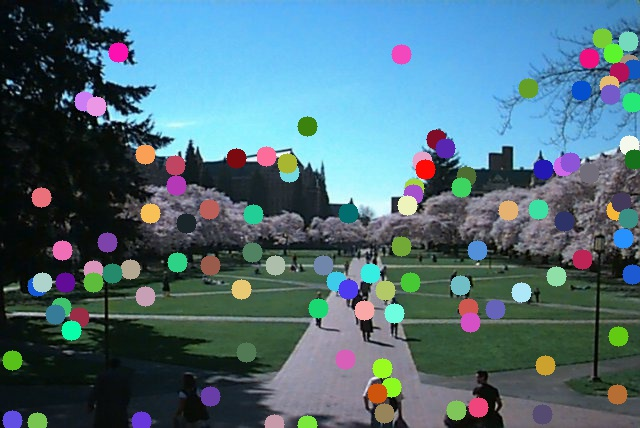
\includegraphics[scale=0.3]{report/p4-3-3-C00}}
		}
		\label{fig:cent00}
	}
	\quad
	\subfloat[X = 6.]{
		{
			\setlength{\fboxsep}{1pt}
			\setlength{\fboxrule}{1pt}
			\fbox{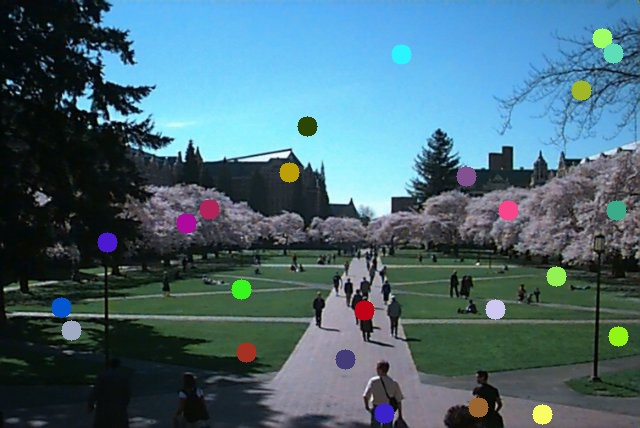
\includegraphics[scale=0.3]{report/p4-3-3-C06}}
		}
		\label{fig:cent06}
	}
	\quad
	\subfloat[X = 10.]{
		{
			\setlength{\fboxsep}{1pt}
			\setlength{\fboxrule}{1pt}
			\fbox{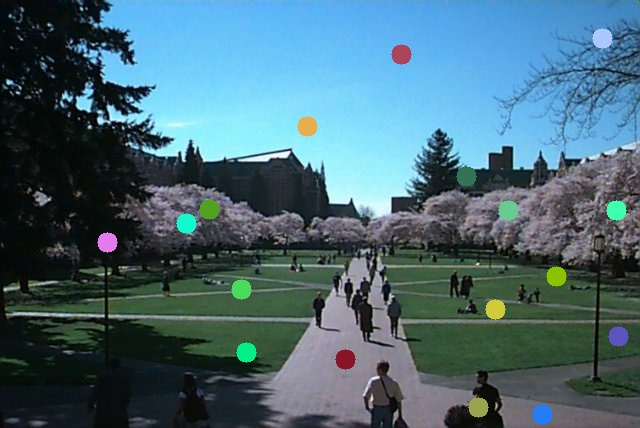
\includegraphics[scale=0.3]{report/p4-3-3-C10}}
		}
		\label{fig:cent10}
	}
	\quad
	\subfloat[X = 20.]{
		{
			\setlength{\fboxsep}{1pt}
			\setlength{\fboxrule}{1pt}
			\fbox{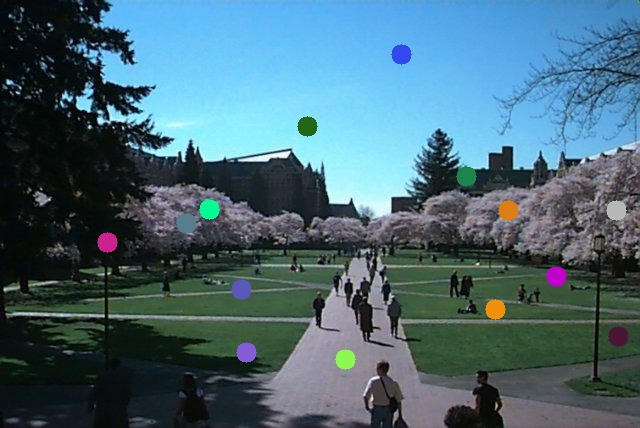
\includegraphics[scale=0.3]{report/p4-3-3-C20}}
		}
		\label{fig:cent20}
	}
	\caption{Centroids of each region calculated with different $X$ values.}
	\label{fig:cent}
\end{figure}

% =========================================================================================================================================================

\newpage

\textbf{\LARGE Question 3 - Distance Measure} \\

In order to create a content-based image retrieval, we developed a distance measurement for our collected descriptors that are based on the regions obtained by the connected components algorithm. The distance formula used was a simple difference method over the features size, mean color and the textures features for each region. Moreover, euclidean distance was used to compute the centroids distances. \\

Every region is described by a single value that is composed by the average between all the differences found in the features descriptors for that region. Two different average processes are taken, the first one between the feature vector for the textures obtained by the co-occurrence matrix, and, the other one is an average operation between all the features for that region. Equations \ref{eq:dist_avr} and \ref{eq:feat_avr} shows the equations for the texture features, and the average of all features, respectively. \\

\begin{equation}
	feat\_weight =  \frac{contrast + correlation + dissimilarity +  energy + entropy}{5}
	\label{eq:dist_avr}
\end{equation}

\begin{equation}
region\_distance =  \frac{size + mean\_color + centroid +  feat\_weight}{4}
\label{eq:feat_avr}
\end{equation}

As images might contain different number of regions, a region is compared to all others and the minimum distance is chosen to represent the region. After determining all the distances for the regions, a average is performed between them, giving a single value to classify the similarity between both images. Smaller values mean more correlation, while higher values describe more distinctive images. These averages are important, they normalize the proportion of each feature. Figure \ref{fig:simpleAvr} shows a result for some queried images. \\

\begin{figure}[!h]
	\centering
	{
		{
			\setlength{\fboxsep}{1pt}
			\setlength{\fboxrule}{1pt}
			\fbox{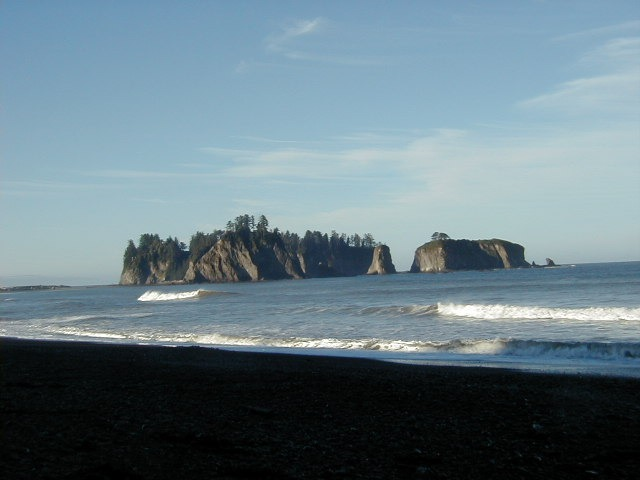
\includegraphics[scale=0.6]{input/beach_2.jpg}}
		}
	}
	\enskip
	{
		{
			\setlength{\fboxsep}{1pt}
			\setlength{\fboxrule}{1pt}
			\fbox{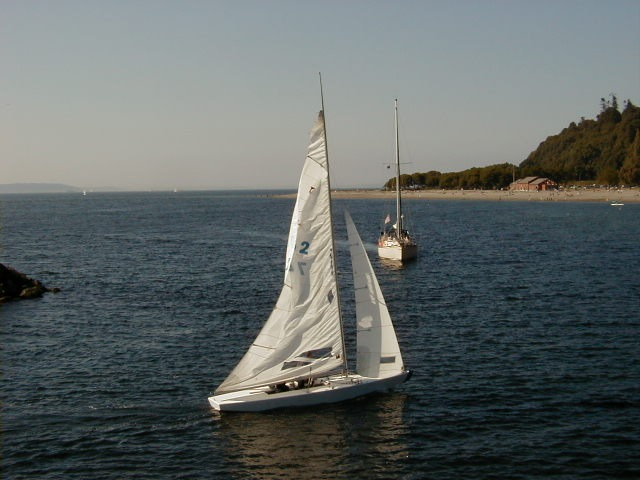
\includegraphics[scale=0.6]{input/boat_2.jpg}}
		}
	}
	\enskip
	{
		{
			\setlength{\fboxsep}{1pt}
			\setlength{\fboxrule}{1pt}
			\fbox{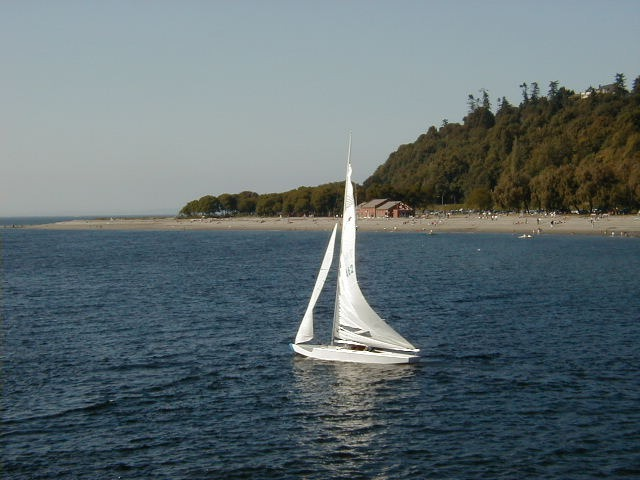
\includegraphics[scale=0.6]{input/boat_5.jpg}}
		}
	}
	\enskip
	{
		{
			\setlength{\fboxsep}{1pt}
			\setlength{\fboxrule}{1pt}
			\fbox{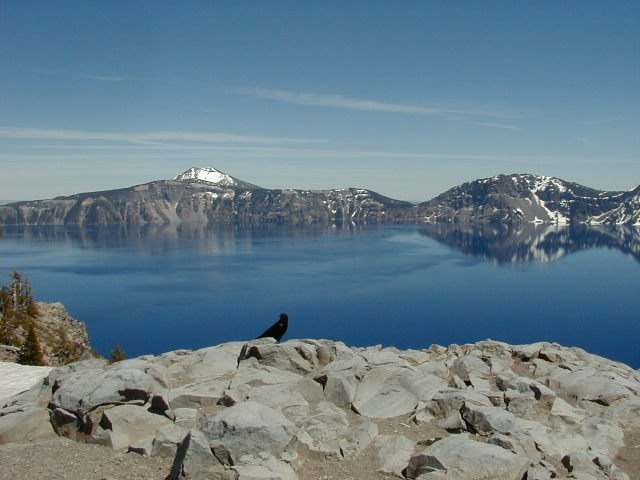
\includegraphics[scale=0.6]{input/crater_1.jpg}}
		}
	}
	\enskip
	
	%-------------------
	
	{
		{
			\setlength{\fboxsep}{1pt}
			\setlength{\fboxrule}{1pt}
			\fbox{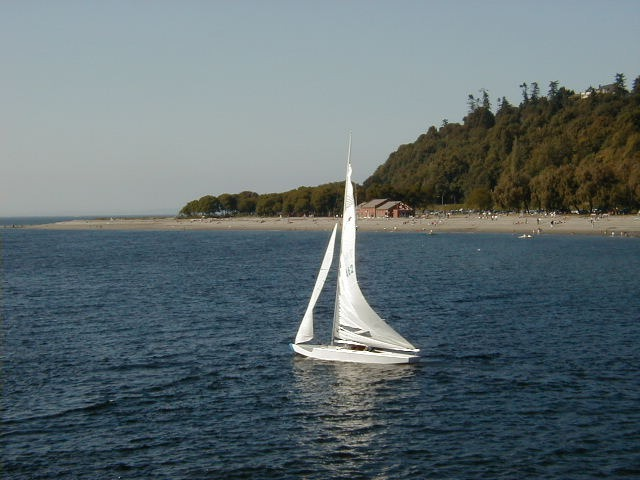
\includegraphics[scale=0.6]{input/boat_5.jpg}}
		}
	}
	\enskip
	{
		{
			\setlength{\fboxsep}{1pt}
			\setlength{\fboxrule}{1pt}
			\fbox{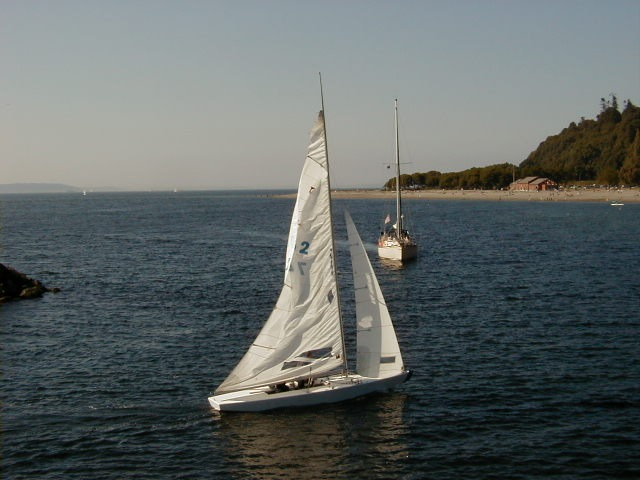
\includegraphics[scale=0.6]{input/boat_2.jpg}}
		}
	}
	\enskip
	{
		{
			\setlength{\fboxsep}{1pt}
			\setlength{\fboxrule}{1pt}
			\fbox{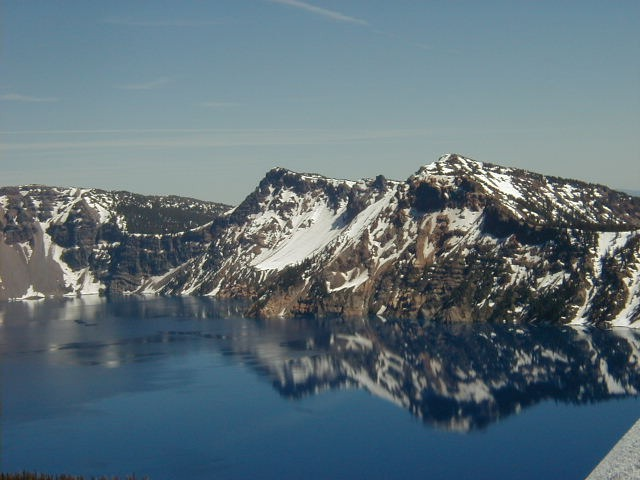
\includegraphics[scale=0.6]{input/crater_5.jpg}}
		}
	}
	\enskip
	{
		{
			\setlength{\fboxsep}{1pt}
			\setlength{\fboxrule}{1pt}
			\fbox{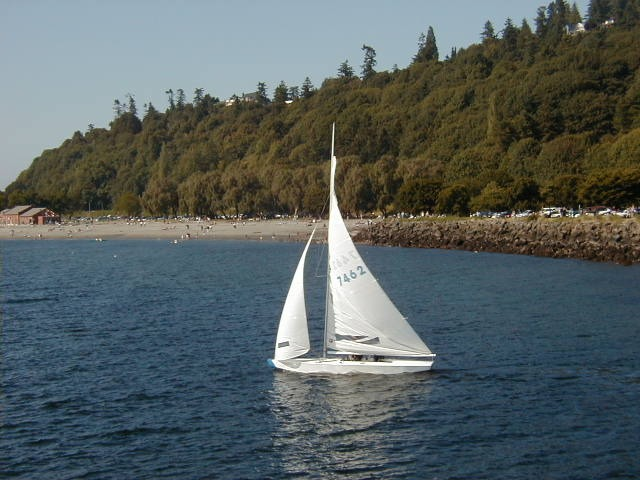
\includegraphics[scale=0.6]{input/boat_4.jpg}}
		}
	}
	\enskip
	%-------------------
	
	{
		{
			\setlength{\fboxsep}{1pt}
			\setlength{\fboxrule}{1pt}
			\fbox{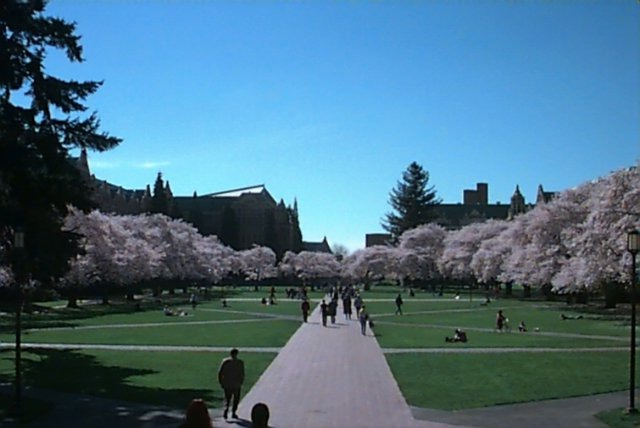
\includegraphics[scale=0.6]{input/cherry_3.jpg}}
		}
	}
	\enskip
	{
		{
			\setlength{\fboxsep}{1pt}
			\setlength{\fboxrule}{1pt}
			\fbox{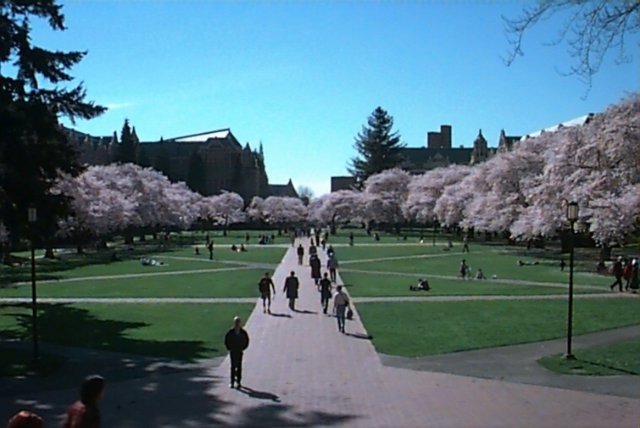
\includegraphics[scale=0.6]{input/cherry_2.jpg}}
		}
	}
	\enskip
	{
		{
			\setlength{\fboxsep}{1pt}
			\setlength{\fboxrule}{1pt}
			\fbox{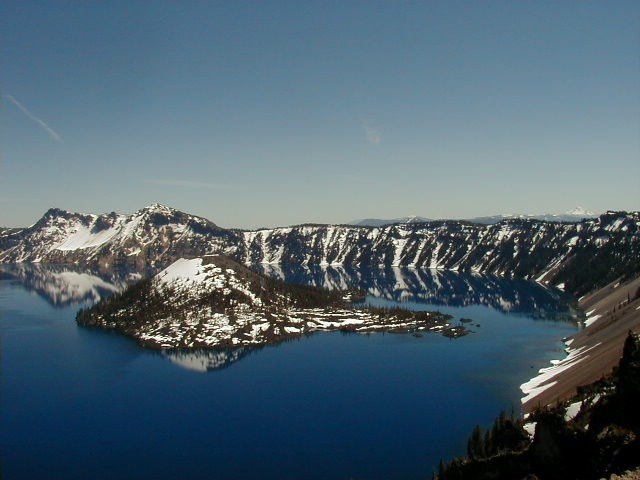
\includegraphics[scale=0.6]{input/crater_3.jpg}}
		}
	}
	\enskip
	{
		{
			\setlength{\fboxsep}{1pt}
			\setlength{\fboxrule}{1pt}
			\fbox{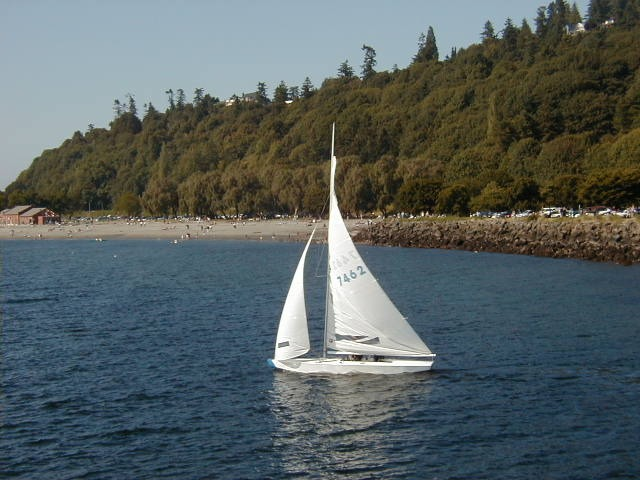
\includegraphics[scale=0.6]{input/boat_4.jpg}}
		}
	}
	\enskip
	%-------------------
	
	{
		{
			\setlength{\fboxsep}{1pt}
			\setlength{\fboxrule}{1pt}
			\fbox{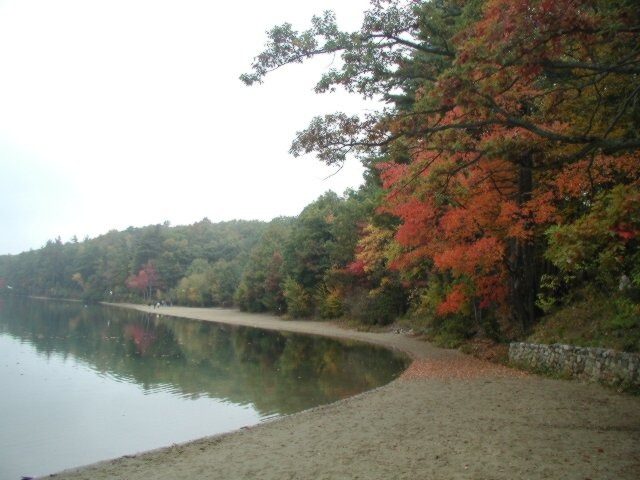
\includegraphics[scale=0.6]{input/pond_2.jpg}}
		}
	}
	\enskip
	{
		{
			\setlength{\fboxsep}{1pt}
			\setlength{\fboxrule}{1pt}
			\fbox{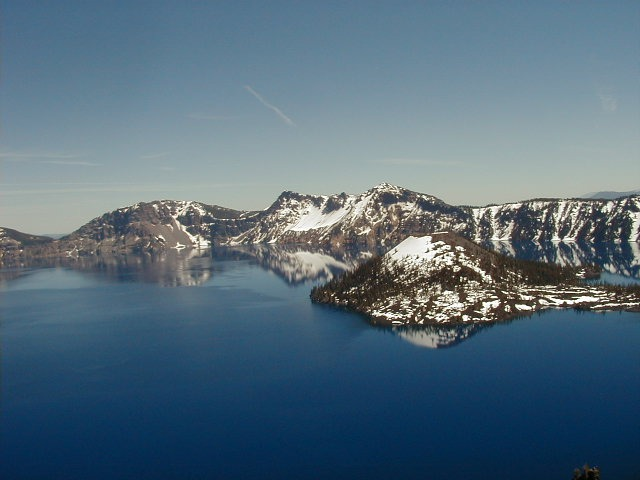
\includegraphics[scale=0.6]{input/crater_2.jpg}}
		}
	}
	\enskip
	{
		{
			\setlength{\fboxsep}{1pt}
			\setlength{\fboxrule}{1pt}
			\fbox{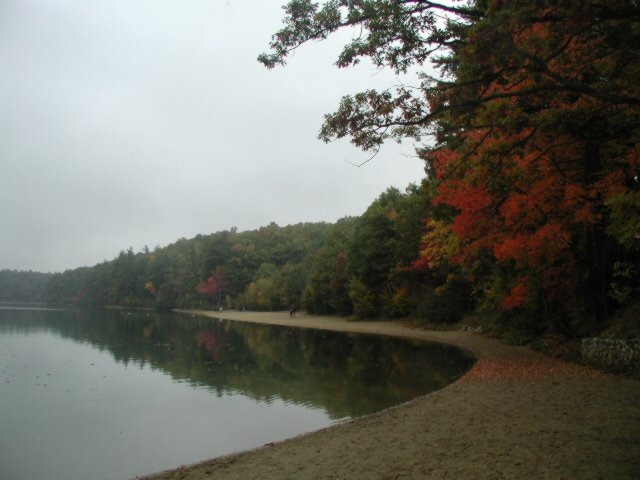
\includegraphics[scale=0.6]{input/pond_3.jpg}}
		}
	}
	\enskip
	{
		{
			\setlength{\fboxsep}{1pt}
			\setlength{\fboxrule}{1pt}
			\fbox{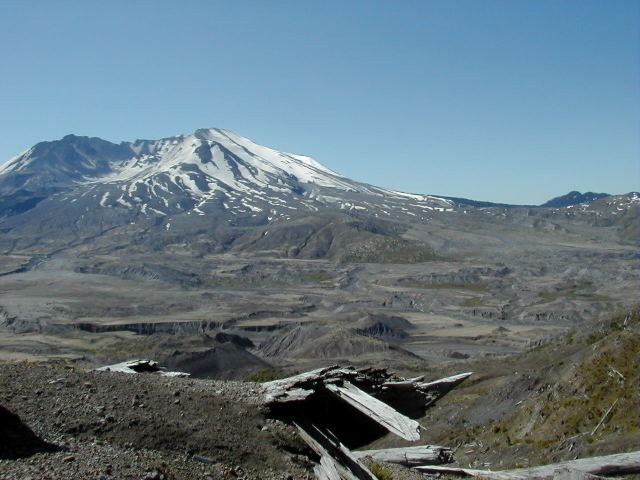
\includegraphics[scale=0.6]{input/stHelens_3.jpg}}
		}
	}\enskip
	
	%-------------------
	
	{
		{
			\setlength{\fboxsep}{1pt}
			\setlength{\fboxrule}{1pt}
			\fbox{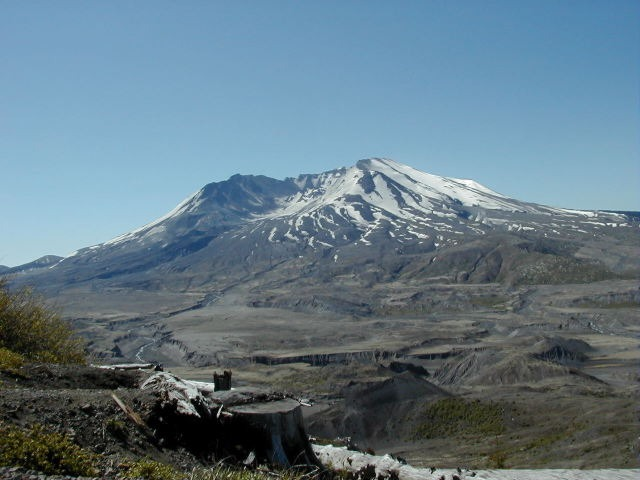
\includegraphics[scale=0.6]{input/stHelens_2.jpg}}
		}
	}
	\enskip
	{
		{
			\setlength{\fboxsep}{1pt}
			\setlength{\fboxrule}{1pt}
			\fbox{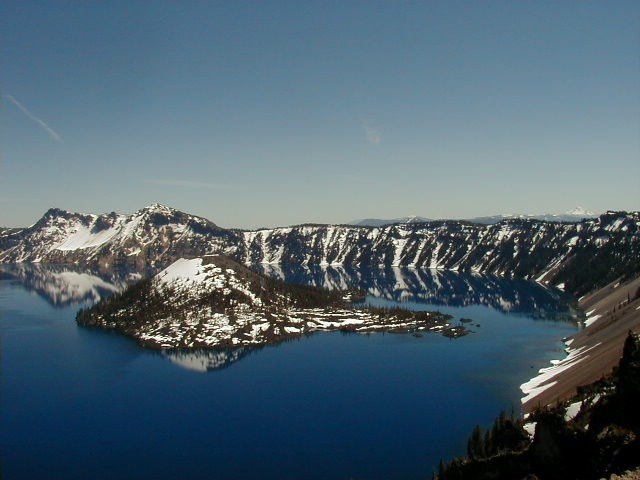
\includegraphics[scale=0.6]{input/crater_3.jpg}}
		}
	}
	\enskip
	{
		{
			\setlength{\fboxsep}{1pt}
			\setlength{\fboxrule}{1pt}
			\fbox{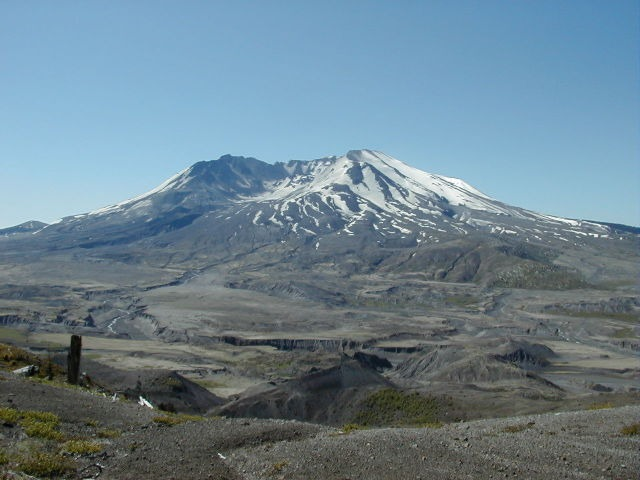
\includegraphics[scale=0.6]{input/stHelens_4.jpg}}
		}
	}
	\enskip
	{
		{
			\setlength{\fboxsep}{1pt}
			\setlength{\fboxrule}{1pt}
			\fbox{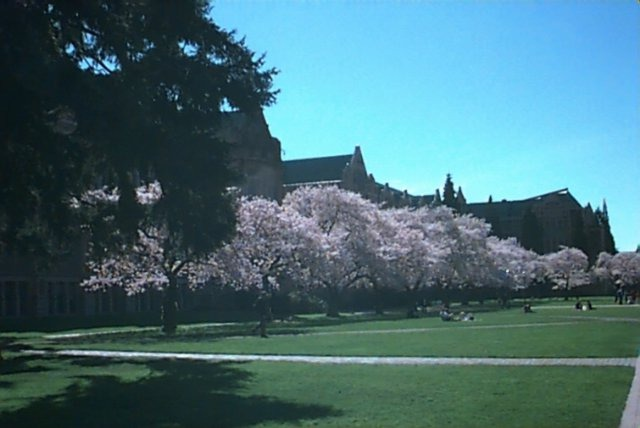
\includegraphics[scale=0.6]{input/cherry_5.jpg}}
		}
	}
	
	%-------------------
	
	{
		{
			\setlength{\fboxsep}{1pt}
			\setlength{\fboxrule}{1pt}
			\fbox{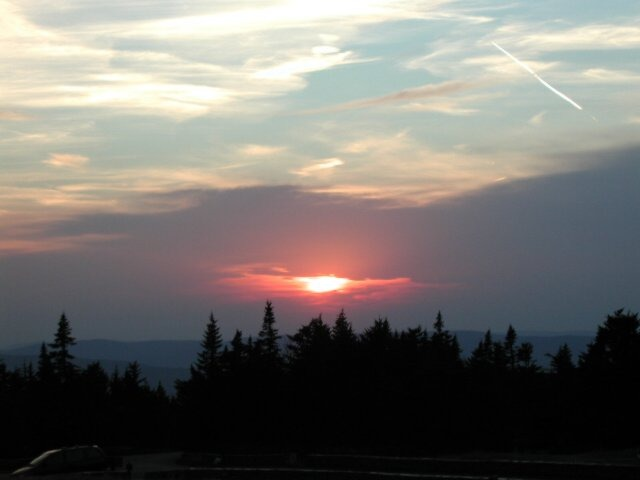
\includegraphics[scale=0.6]{input/sunset1_2.jpg}}
		}
	}
	\enskip
	{
		{
			\setlength{\fboxsep}{1pt}
			\setlength{\fboxrule}{1pt}
			\fbox{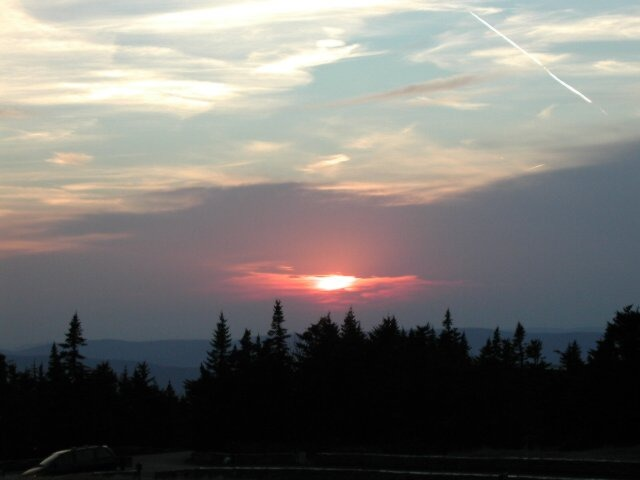
\includegraphics[scale=0.6]{input/sunset1_3.jpg}}
		}
	}
	\enskip
	{
		{
			\setlength{\fboxsep}{1pt}
			\setlength{\fboxrule}{1pt}
			\fbox{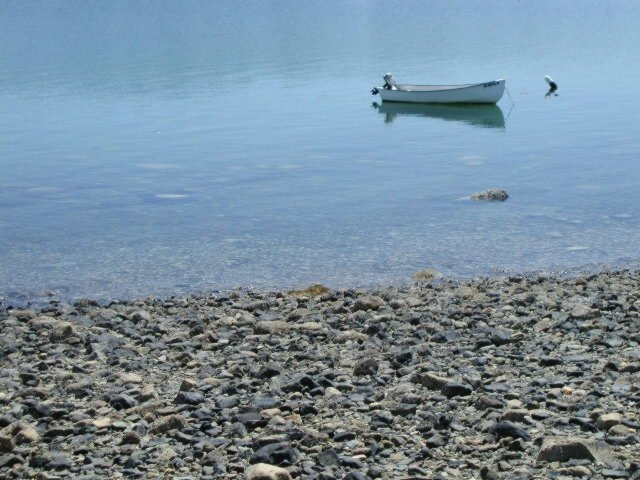
\includegraphics[scale=0.6]{input/boat_1.jpg}}
		}
	}
	\enskip
	{
		{
			\setlength{\fboxsep}{1pt}
			\setlength{\fboxrule}{1pt}
			\fbox{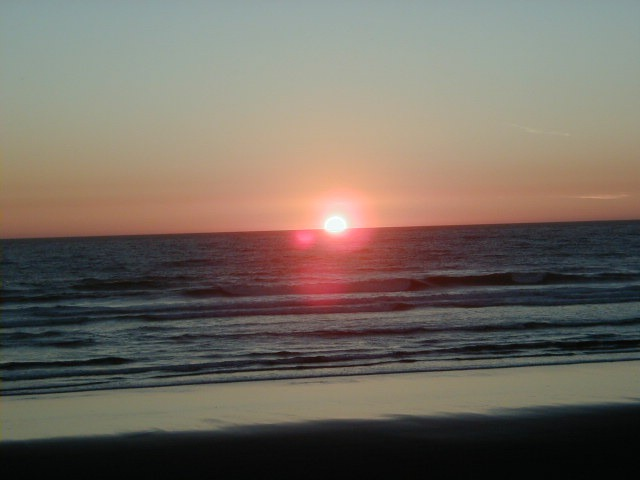
\includegraphics[scale=0.6]{input/sunset2_5.jpg}}
		}
	}
	
	%-------------------
	
	{
		{
			\setlength{\fboxsep}{1pt}
			\setlength{\fboxrule}{1pt}
			\fbox{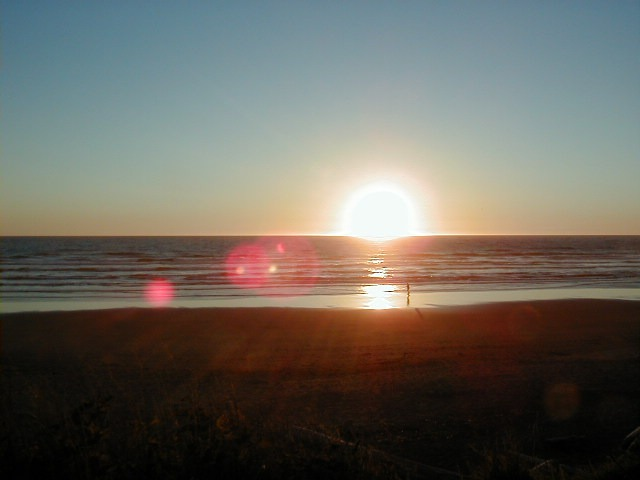
\includegraphics[scale=0.6]{input/sunset2_2.jpg}}
		}
	}
	\enskip
	{
		{
			\setlength{\fboxsep}{1pt}
			\setlength{\fboxrule}{1pt}
			\fbox{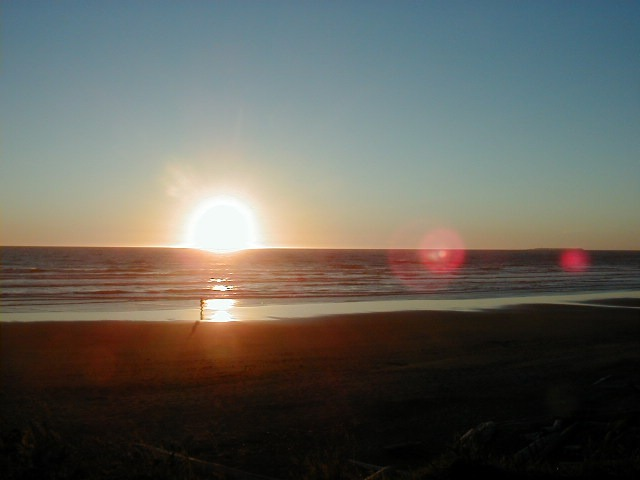
\includegraphics[scale=0.6]{input/sunset2_3.jpg}}
		}
	}
	\enskip
	{
		{
			\setlength{\fboxsep}{1pt}
			\setlength{\fboxrule}{1pt}
			\fbox{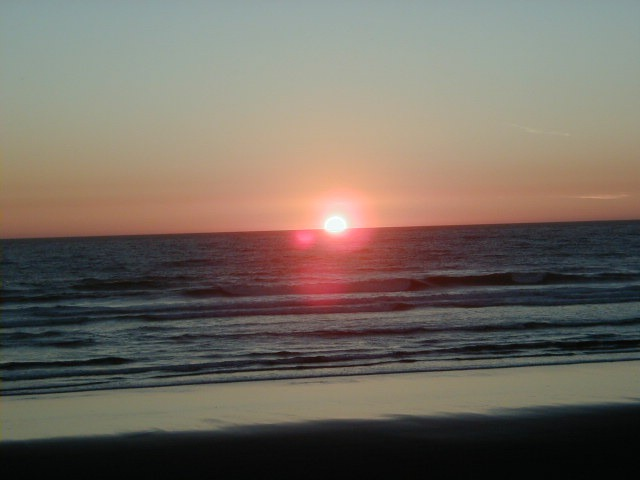
\includegraphics[scale=0.6]{input/sunset2_5.jpg}}
		}
	}
	\enskip
	{
		{
			\setlength{\fboxsep}{1pt}
			\setlength{\fboxrule}{1pt}
			\fbox{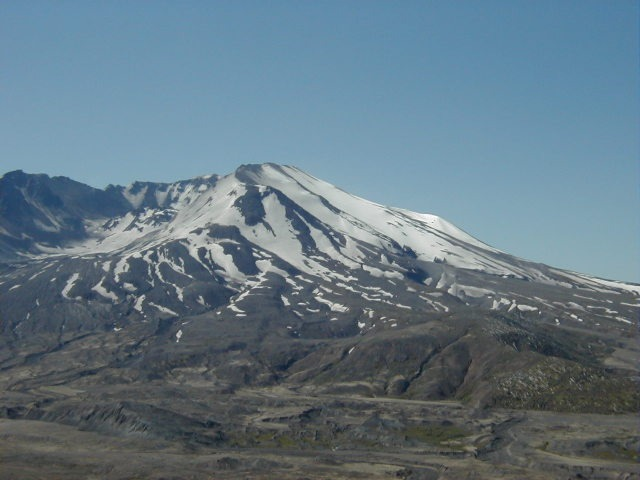
\includegraphics[scale=0.6]{input/stHelens_5.jpg}}
		}
	}
	
		
	\caption{Retrieved images using the left column as queries, in order the columns are Queried image, 1º rank, 2º rank, and 3º rank.}
	\label{fig:simpleAvr}
\end{figure}

Figure \ref{fig:simpleAvr} shows that in some cases the results are pretty good, for example for the query (boat\_5) which is represented by the second row, two of the images has a boat in it. Moreover, the second ranked image, is also composed of a land and a river. However, in the third row the second ranked (crater\_3) image is not so similar to the queried image (cherry\_3). \\ 

Those results shows us that large regions are being largely used for comparing the images, however, it is hard to choose the best features to use. In this way, in order to create a more robust system we decided to change the simple average to a weighted average (in both averages processes), this way we could optimize the weights for the average choosing the best weights for our dataset. Equations \ref{eq:complex_dist} and \ref{eq:complex_feat} shows the new average processes. \\

\begin{equation}
feat\_weight =  \frac{w_1 * contrast + w_2 * correlation + w_3 * dissimilarity + w_4 *  energy + w_5 * entropy}{w_1 + w_2 + w_3 + w_4 + w_5}
\label{eq:complex_dist}
\end{equation}

\begin{equation}
region\_distance =  \frac{w_6 * size + w_7 * mean\_color + w_8 * centroid +  w_9 * feat\_weight}{w_6 + w_7 + w_8 + w_9}
\label{eq:complex_feat}
\end{equation}


In order to optimize these weights, the mean distance between one specified image with all images in the same class were used. We searched in a space between 0 and 2 for each feature, as we have 9 values a total of 19683 different weights were tested and the following weights had the best results (smaller mean distance for images of the same class): $w_1 = 0, \ w_2 = 0, \ w_3 = 0, \ w_4 = 0, \ w_5 = 1, \ w_6 = 1, \ w_7 = 1, \ w_8 = 1, \ w_9 = 1 \ $. These weights shows that the optimization decided that some of the co-occurrence features were not improving the overall result, the only feature used was entropy which seems to not help a lot the algorithm to not be based just on color intensity. Figure \ref{fig:complexAvr} shows the retrieved images for the same queries as before. \\

\begin{figure}[!h]
	\centering
	{
		{
			\setlength{\fboxsep}{1pt}
			\setlength{\fboxrule}{1pt}
			\fbox{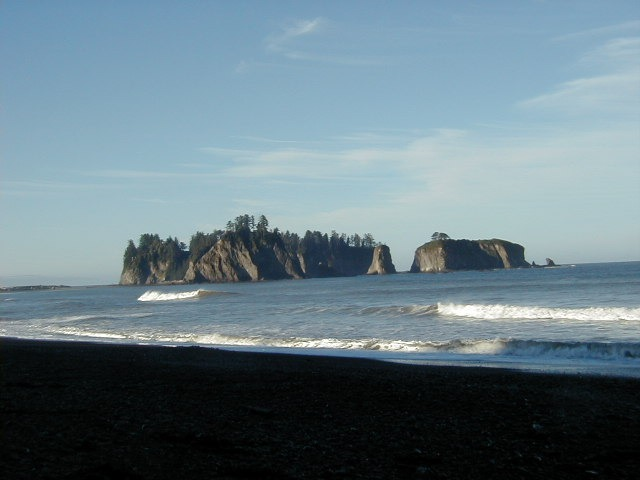
\includegraphics[scale=0.6]{input/beach_2.jpg}}
		}
	}
	\enskip
	{
		{
			\setlength{\fboxsep}{1pt}
			\setlength{\fboxrule}{1pt}
			\fbox{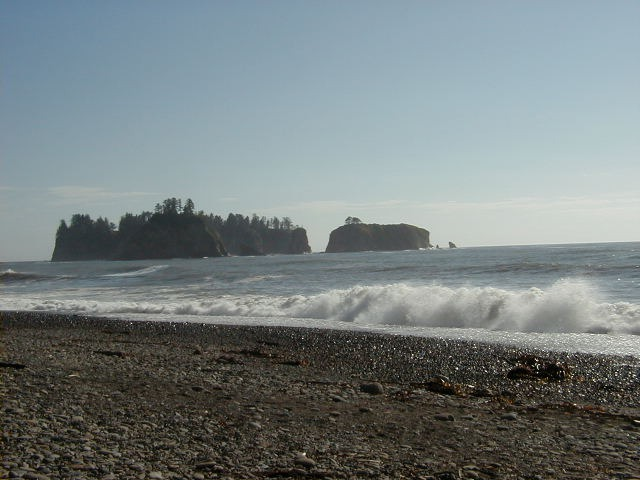
\includegraphics[scale=0.6]{input/beach_1.jpg}}
		}
	}
	\enskip
	{
		{
			\setlength{\fboxsep}{1pt}
			\setlength{\fboxrule}{1pt}
			\fbox{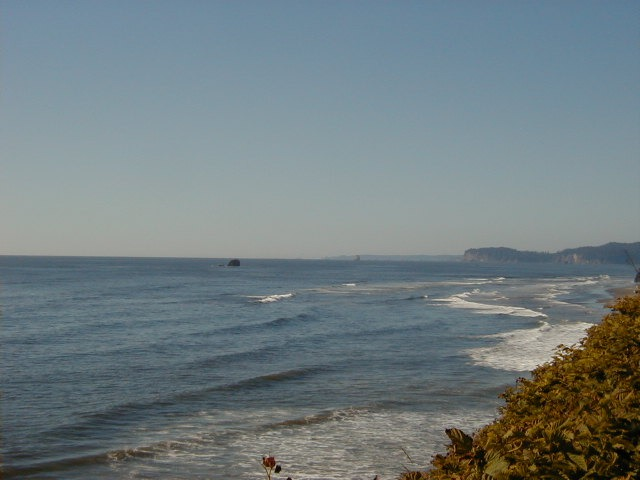
\includegraphics[scale=0.6]{input/beach_5.jpg}}
		}
	}
	\enskip
	{
		{
			\setlength{\fboxsep}{1pt}
			\setlength{\fboxrule}{1pt}
			\fbox{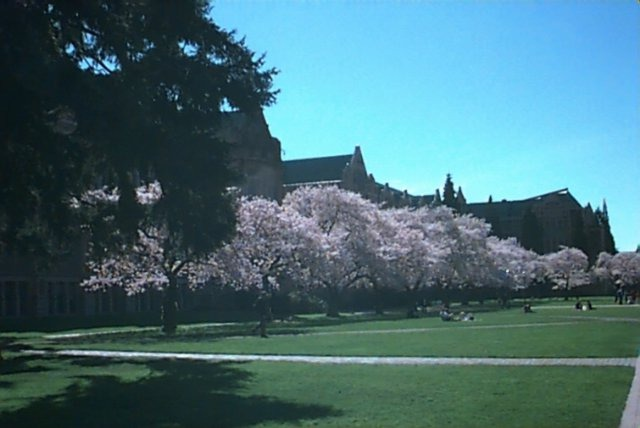
\includegraphics[scale=0.6]{input/cherry_5.jpg}}
		}
	}
	\enskip
	
	%-------------------
	
	{
		{
			\setlength{\fboxsep}{1pt}
			\setlength{\fboxrule}{1pt}
			\fbox{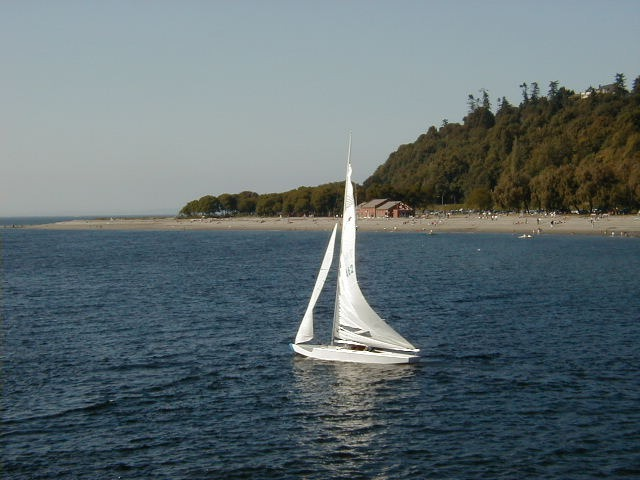
\includegraphics[scale=0.6]{input/boat_5.jpg}}
		}
	}
	\enskip
	{
		{
			\setlength{\fboxsep}{1pt}
			\setlength{\fboxrule}{1pt}
			\fbox{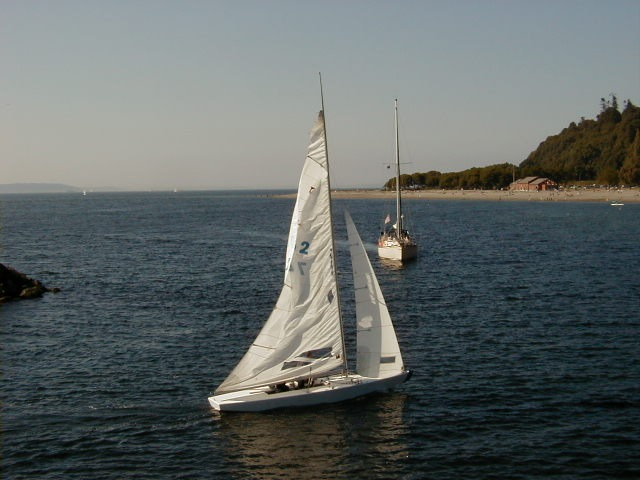
\includegraphics[scale=0.6]{input/boat_2.jpg}}
		}
	}
	\enskip
	{
		{
			\setlength{\fboxsep}{1pt}
			\setlength{\fboxrule}{1pt}
			\fbox{\includegraphics[scale=0.6]{input/crater_5.jpg}}
		}
	}
	\enskip
	{
		{
			\setlength{\fboxsep}{1pt}
			\setlength{\fboxrule}{1pt}
			\fbox{\includegraphics[scale=0.6]{input/stHelens_2.jpg}}
		}
	}
	\enskip
	%-------------------
	
	{
		{
			\setlength{\fboxsep}{1pt}
			\setlength{\fboxrule}{1pt}
			\fbox{\includegraphics[scale=0.6]{input/cherry_3.jpg}}
		}
	}
	\enskip
	{
		{
			\setlength{\fboxsep}{1pt}
			\setlength{\fboxrule}{1pt}
			\fbox{\includegraphics[scale=0.6]{input/cherry_1.jpg}}
		}
	}
	\enskip
	{
		{
			\setlength{\fboxsep}{1pt}
			\setlength{\fboxrule}{1pt}
			\fbox{\includegraphics[scale=0.6]{input/stHelens_5.jpg}}
		}
	}
	\enskip
	{
		{
			\setlength{\fboxsep}{1pt}
			\setlength{\fboxrule}{1pt}
			\fbox{\includegraphics[scale=0.6]{input/boat_3.jpg}}
		}
	}
	\enskip
	%-------------------
	
	{
		{
			\setlength{\fboxsep}{1pt}
			\setlength{\fboxrule}{1pt}
			\fbox{\includegraphics[scale=0.6]{input/pond_2.jpg}}
		}
	}
	\enskip
	{
		{
			\setlength{\fboxsep}{1pt}
			\setlength{\fboxrule}{1pt}
			\fbox{\includegraphics[scale=0.6]{input/stHelens_4.jpg}}
		}
	}
	\enskip
	{
		{
			\setlength{\fboxsep}{1pt}
			\setlength{\fboxrule}{1pt}
			\fbox{\includegraphics[scale=0.6]{input/stHelens_5.jpg}}
		}
	}
	\enskip
	{
		{
			\setlength{\fboxsep}{1pt}
			\setlength{\fboxrule}{1pt}
			\fbox{\includegraphics[scale=0.6]{input/beach_3.jpg}}
		}
	}\enskip
	
	%-------------------
	
	{
		{
			\setlength{\fboxsep}{1pt}
			\setlength{\fboxrule}{1pt}
			\fbox{\includegraphics[scale=0.6]{input/stHelens_2.jpg}}
		}
	}
	\enskip
	{
		{
			\setlength{\fboxsep}{1pt}
			\setlength{\fboxrule}{1pt}
			\fbox{\includegraphics[scale=0.6]{input/crater_1.jpg}}
		}
	}
	\enskip
	{
		{
			\setlength{\fboxsep}{1pt}
			\setlength{\fboxrule}{1pt}
			\fbox{\includegraphics[scale=0.6]{input/stHelens_4.jpg}}
		}
	}
	\enskip
	{
		{
			\setlength{\fboxsep}{1pt}
			\setlength{\fboxrule}{1pt}
			\fbox{\includegraphics[scale=0.6]{input/pond_3.jpg}}
		}
	}
	
	%-------------------
	
	{
		{
			\setlength{\fboxsep}{1pt}
			\setlength{\fboxrule}{1pt}
			\fbox{\includegraphics[scale=0.6]{input/sunset1_2.jpg}}
		}
	}
	\enskip
	{
		{
			\setlength{\fboxsep}{1pt}
			\setlength{\fboxrule}{1pt}
			\fbox{\includegraphics[scale=0.6]{input/sunset1_3.jpg}}
		}
	}
	\enskip
	{
		{
			\setlength{\fboxsep}{1pt}
			\setlength{\fboxrule}{1pt}
			\fbox{\includegraphics[scale=0.6]{input/sunset1_1.jpg}}
		}
	}
	\enskip
	{
		{
			\setlength{\fboxsep}{1pt}
			\setlength{\fboxrule}{1pt}
			\fbox{\includegraphics[scale=0.6]{input/boat_4.jpg}}
		}
	}
	
	%-------------------
	
	{
		{
			\setlength{\fboxsep}{1pt}
			\setlength{\fboxrule}{1pt}
			\fbox{\includegraphics[scale=0.6]{input/sunset2_2.jpg}}
		}
	}
	\enskip
	{
		{
			\setlength{\fboxsep}{1pt}
			\setlength{\fboxrule}{1pt}
			\fbox{\includegraphics[scale=0.6]{input/stHelens_2.jpg}}
		}
	}
	\enskip
	{
		{
			\setlength{\fboxsep}{1pt}
			\setlength{\fboxrule}{1pt}
			\fbox{\includegraphics[scale=0.6]{input/sunset2_3.jpg}}
		}
	}
	\enskip
	{
		{
			\setlength{\fboxsep}{1pt}
			\setlength{\fboxrule}{1pt}
			\fbox{\includegraphics[scale=0.6]{input/pond_3.jpg}}
		}
	}
	
	
	\caption{Retrieved images using weights, in order the columns are queried image, 1º rank, 2º rank, and 3º rank.}
	\label{fig:complexAvr}
\end{figure}

Figure \ref{fig:complexAvr} shows some improvements for some classes as the beach class, however, it is still guessing some weird results like the third rank for the beach query (cherry\_5). It is also clear that the system is retrieving more similar images in the higher ranks compared to the other approach. Another important note is that the algorithm is highly related with colors, which some times confuses different image because of a large amount of blue sky or ocean. \\

In order to retrieve better results, we could have searched for betters weights in a larger space domain. However, this search is highly computer expensive. A better approach would be to use different features extractor, which are not too related with colors. A SIFT or HOG descriptor for each region could be applied, but it would turn the algorithm more time consuming. 


\end{document}
